\section{Préambule}
Le choix du système de base de données s'est porté sur \texttt{MariaDB}, un \textit{fork} de \texttt{MySQL}. Cela vient de notre volonté à utiliser des logiciels \href{https://mariadb.com/database-topics/mariadb-vs-mysql/}{non propriétaire} au sein de ce projet.


\section{Installation du serveur MariaDB}

\subsection{Installation des paquets}
L'installation de la base de données sur notre machine virtuelle sous \texttt{Ubuntu Server}, se fait par un script bash \texttt{installDB.sh} à lancer avec \texttt{sudo}.

\begin{minted}{bash}
admin@serveur> sudo ./installDB.sh
\end{minted}

Il va d'abord mettre à jour la liste des paquets afin de récupérer les dernières versions de ces derniers contenant les mises à jour de sécurité les plus récentes. Dans notre cas, nous voulons installer le serveur de base de données, mais également accéder à la base pour effectuer des opérations. Il se trouve que l'installation du paquet du serveur \texttt{mariadb-server} lance automatiquement celles des paquets \texttt{mariadb-client} et \texttt{mariadb-common}, on va donc pouvoir simplement installer ce paquet.\\\\ 

\subsection{Installation sécurisé}
Après ces opérations, le script va lancer l'installation en mode sécurisé, afin d'ajouter des options de sécurité à notre serveur de base de données.\\\\
Il faudra répondre \color{green}Y\color{black} (oui) ou \color{red}n \color{black}(non) pour activer ou désactiver ces options.\\\\
\begin{center}
    Voici nos recommandations :
\end{center}

\begin{itemize}
    \item Demande le \texttt{mot de passe root} MariaDB : Pressez \textbf{Enter} pour passer car il n'existe pas encore.
    \item Utilisation de \texttt{sockets d'authentification} : \color{red}\textbf{n}  \color{black}, Ce ne sera pas utile, on désactive le compte root en remote par la suite.
    \item Changer le mot de passe root : \color{red}\textbf{n} \color{black}, Encore une fois, le compte root sera uniquement accessible via un sudo depuis le serveur où est installé \texttt{MariaDB Server} et donc déjà protégé par le mot de passe du compte Linux.
    \item Suppression des utilisateurs anonymes : \color{green}\textbf{Y} \color{black}, On désactive ces comptes permettant une connexion non sécurisée à la base. Nous allons créer un utilisateur pour le projet par la suite.
    \item Désactiver la connexion à distance sur root : \color{green}\textbf{Y} \color{black}, C'est l'un des points les plus \textbf{importants} car il impacte les choix précédents.
    \item Suppression des bases de tests et leur accès : \color{green}\textbf{Y}\color{black}, Nous allons être dans un contexte de production et donc ces bases ne nous servent pas.
    \item Rafraîchir la table des privilèges : \color{green}\textbf{Y} \color{black}, Pour prendre en compte nos options de sécurité dès à présent.
\end{itemize}
Par la suite, on pourra vérifier l'état de notre serveur \texttt{MariaDB} avec la commande :
\begin{minted}{bash}
admin@serveur> sudo systemctl status mariadb.service
\end{minted}
 Pour finir, le script va nous connecter au serveur MariaDB sur le compte root afin de passer à la mise en place de la base 2DMatrix. En effet, vu que l'on a décidé précédemment de ne pas mettre de mot de passe au compte root de MariaDB, on se connecte sans mot de passe (à part celui du compte Linux pour \texttt{sudo}) à la base en tant qu'administrateur.
 
 \section{Installation de la base 2DMATRIX\_DATABASE}
\subsection{Création de la base et de l'utilisateur}
Encore une fois, on va exécuter un script (\textit{create\_base.sql}) directement dans la console MySQL en tapant :
\begin{minted}{SQL}
root@localhost > @/chemin_vers_script/create_base.sql
\end{minted}
Ce dernier va commencer par créer la base \texttt{2DMATRIX\_DATABASE} et se placer dans cette base. Ensuite, on va créer 
un utilisateur \texttt{2DMatrix@localhost} qui pourra se connecter à la base du projet. Il faut changer le mot de passe dans le script au niveau de la ligne \texttt{CREATE USER...} pour y mettre le sien une fois que le script se trouve en sécurité sur le serveur. Ensuite, le script va donner l'ensemble des privilèges à notre utilisateur sur la base \texttt{2DMATRIX\_DATABASE} et mettre à jour la table des droits du serveur \texttt{MariaDB}.\\\\
\textbf{Remarque} : Le script SQL possède des lignes \texttt{DROP ...}. Il faut donc faire attention si la base a été installée précédemment et que les tables contiennent des données. Les éléments supprimés pour être recréés sont : l'utilisateur et les deux tables \texttt{ORGANIZATION} et \texttt{USER\_ACCOUNT} du projet. Le script ne supprime pas la base \texttt{2DMATRIX\_DATABASE}, il se contente de la créer si elle n'existe pas. Il faut donc bien prendre en compte ces deux points.

\subsection{Création des tables}
\subsection{Schémas}
\begin{center}
    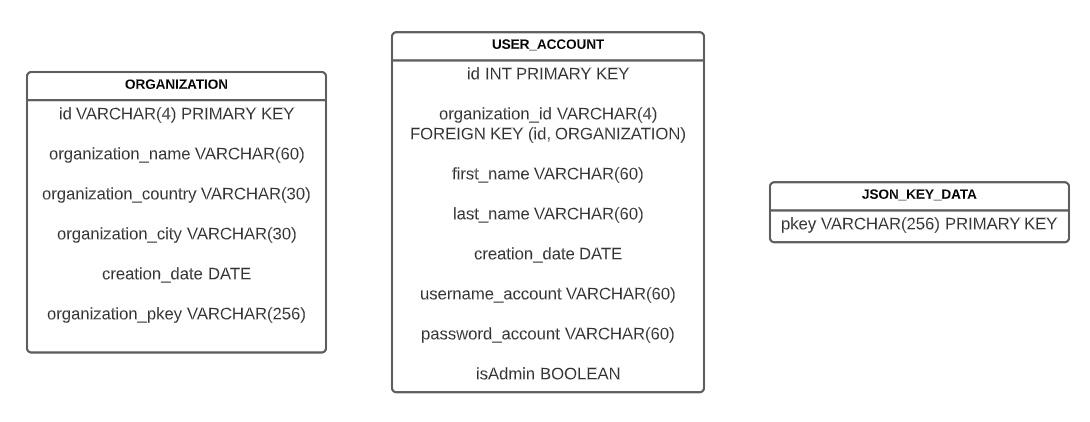
\includegraphics[scale=0.6]{imgs/bdd.PNG}\\
    \textit{Tables des organisations, des comptes utilisateurs (utilisateurs organisme et administrateurs organisme) et de la clé de signature du fichier JSON. (TSL / Blackliste)}
\end{center}

\subsection{Les Tables du projet}
En ce qui concerne les tables, la première (\texttt{ORGANIZATION}), permet de stocker les différentes organisations étant en réalité les autorités de certifications. Cette table va contenir différentes informations générales sur l'organisation comme le nom, la date de création, etc... mais surtout la clé permettant de signer les données d'un DataMatrix 2D-Doc, créé pour certifier un document administratif.\\\\
La seconde table (\texttt{USER\_ACCOUNT}), sert à stocker les différents comptes utilisateurs des organisations. Cette table contient, comme la précédente, les informations de la personne, mais également un booléen \textit{isAdmin} qui permet de distinguer les comptes \textit{administrateur organisme} des comptes \textit{utilisateur organisme} afin de les diriger sur le bon outil, à savoir, \texttt{2DMatrix-Manage} ou \texttt{2DMatrix-Create} respectivement.\\\\
Pour finir, la table \texttt{JSON\_KEY\_DATA} contient simplement une colonne et une ligne servant à stocker la clé privée qui signe notre fichier json. (\texttt{TSL / Blackliste})\\\\

\section{Utilisation de la base de données par 2DMatrix}

\subsection{Connexion à la base}

Pour la connexion à la base de données, on utilise une classe PHP qui récupère une connexion \texttt{PDO} sur notre base. De là, on effectue des requêtes pour l'ensemble des opérations à effectuer. (\texttt{SELECT}, \texttt{UPDATE}, \texttt{DELETE}, ...). 

L'utilisation de PDO permet d'utiliser les requêtes préparées et est un bon remplaçant de \texttt{mysqli}. (déprécié)

Notre classe PHP (\texttt{DB}) se sert d'une classe \texttt{Config} qui va récupérer des valeurs de configurations dans notre fichier \texttt{DBconfig.json} permettant donc une connexion dynamique en fonction de ce dernier au sein de l'application.

\subsection{Ajout de sécurités}

L'utilisation de requêtes préparées permet d'éviter certaines attaques comme les Injections SQL et sont donc constamment utilisées dans notre code pour les appels à la base de données. 

Pour ajouter une surcouche de sécurité, on déspécialise les informations récupérées dans les formulaires avec la fonction \texttt{htmlspecialchars()}.

Également, les données sensibles comme les mots de passes des comptes utilisateurs et administrateur organisme sont ajoutés dans la base en haché \texttt{SHA256}.
\newpage
\section{Annexes}
\subsection{Script bash d'installation de MariaDB Server}
\begin{minted}{bash}
#!/bin/bash

# Mise à jour
apt update

# Installation du serveur
apt install mariadb-server  

# Option de sécurité mysql
mysql_secure_installation

# Démarrage sql
mariadb -u root
\end{minted}

\subsection{Script MySQL d'installation de la base de données du projet}

\begin{minted}{sql}
--
-- MySQL Script for DataBase of 2DMatrix Project
-- 

CREATE DATABASE IF NOT EXISTS 2DMATRIX_DATABASE;
USE 2DMATRIX_DATABASE;

DROP USER IF EXISTS '2DMatrix'@'localhost';

CREATE USER '2DMatrix'@'localhost' 
IDENTIFIED BY 'my_very_strong_password_2DMatrix';

GRANT ALL PRIVILEGES ON 2DMATRIX_DATABASE.* 
TO '2DMatrix'@'localhost';

FLUSH PRIVILEGES;

DROP TABLE IF EXISTS USER_ACCOUNT;
DROP TABLE IF EXISTS ORGANIZATION;

CREATE TABLE ORGANIZATION (
    id VARCHAR(4) NOT NULL,
    organization_name VARCHAR(60) NOT NULL,
    organization_country VARCHAR(30) NOT NULL,
    organization_city VARCHAR(30) NOT NULL,
    creation_date DATE,
    organization_pkey VARCHAR(256) NOT NULL,
    PRIMARY KEY (id));

CREATE TABLE USER_ACCOUNT (
    id INT NOT NULL AUTO_INCREMENT,
    organization_id VARCHAR(4) NOT NULL,
    first_name VARCHAR(60) NOT NULL,
    last_name VARCHAR(60) NOT NULL,
    creation_date DATE,
    username_account VARCHAR(30) NOT NULL,
    password_account VARCHAR(255) NOT NULL,
    isAdmin BOOLEAN NOT NULL,
    PRIMARY KEY (id),
    CONSTRAINT fk_user_account FOREIGN KEY
    USER_ACCOUNT(organization_id) REFERENCES
    ORGANIZATION(id));

CREATE TABLE JSON_KEY_DATA (
    json_pkey VARCHAR(256) NOT NULL,
    PRIMARY KEY (json_pkey)
);
\end{minted}